\documentclass[11pt]{article}

\usepackage[a4paper]{geometry}
\geometry{left=2.0cm,right=2.0cm,top=3cm,bottom=2.5cm}
\usepackage{setspace}
\setstretch{1.5}
\usepackage{ctex}
\usepackage{amsmath,amsfonts,graphicx,amssymb,bm,amsthm}
\usepackage{algorithm,algorithmicx}
\usepackage[noend]{algpseudocode}
\usepackage{fancyhdr}
\usepackage{booktabs}
\usepackage{array}
\usepackage{float}
\usepackage{listings}
\usepackage{xcolor}
\usepackage{url}

\lstset{
	language=Python,
	basicstyle=\ttfamily\small,
	numbers=left,
	numberstyle=\tiny\color{teal!70!black},
	showstringspaces=false,
	breaklines=true,
	frame=single,
	rulecolor=\color{black},
	framerule=0.6pt,
	framesep=4pt,
	xleftmargin=6pt,
	backgroundcolor=\color{gray!4},
	columns=fullflexible,
	keywordstyle=\bfseries\color{blue!70!black},
	commentstyle=\itshape\color{green!50!black},
	stringstyle=\color{red!60!black},
	identifierstyle=\color{violet!70!black},
	emphstyle=\bfseries\color{orange!80!black},
	tabsize=4
}
\newcolumntype{M}[1]{>{\centering\arraybackslash}m{#1}}
\setlength{\headheight}{14pt}

\newcommand{\transbox}[4]{
	\begin{center}
		\fcolorbox{black!25}{gray!4}{
			\begin{minipage}{0.92\linewidth}
				\textbf{#1}\par\vspace{0.25em}
				\textbf{源句：}#2\par
				\textbf{模型译文：}#3\par
				\textbf{参考译文：}#4
			\end{minipage}
		}
	\end{center}
}

\begin{document}
	\pagestyle{fancy}
	\lhead{\kaishu 中国科学院大学}
	\chead{}
	\rhead{\kaishu 2026年春季学期\qquad 深度学习}
	
	\begin{center}
		{\LARGE \bf 实验四：基于Transformer的神经机器翻译}
	\end{center}
	\begin{center}
		\large\kaishu{尧祥临 202518023406038 前沿交叉科学学院}
	\end{center}

	\section{任务介绍}
	本次实验的任务是基于Transformer实现中英神经机器翻译模型，并在测试集上使用BLEU-4作为主要评价指标。实验数据来自NiuTrans开源中英平行语料，训练集包含中文和英文各100000行，开发集包含400个句对，测试集包含1000个中文句子，并提供对应英文参考译文用于计算BLEU。

	机器翻译与前面几个分类或语言建模实验不同。分类任务的输出空间固定，评价指标通常只关心预测类别是否正确；翻译任务的输出是变长文本序列，同一个中文句子可能存在多种合理英文表达。因此，本实验不仅需要构造编码器-解码器结构，还需要在训练时使用teacher forcing，在推理时使用自回归解码，并通过BLEU衡量模型译文和参考译文之间的n-gram匹配程度。

	\section{数据处理}
	原始训练集以两个文件保存，中文和英文按行一一对应。中文语料已经完成分词，英文语料也已经转为小写并按空格切分，因此代码中直接使用空格作为token边界。开发集和参考译文文件采用``中文行、空行、英文行''的交错格式，读取时需要先去除空行，再每两行组成一个句对。

	预处理阶段分别根据训练集中文和英文token构造源语言词表与目标语言词表。词表保留出现次数不少于2的token，并限制最大大小为30000。为了支持批量训练和自回归生成，词表中额外加入\texttt{<pad>}、\texttt{<bos>}、\texttt{<eos>}和\texttt{<unk>}四个特殊符号。每个句子编码时在首尾分别加入\texttt{<bos>}和\texttt{<eos>}，超过最大长度80的句子进行截断。

	\begin{lstlisting}
def encode_pairs(pairs, src_vocab, tgt_vocab, max_len):
    encoded = []
    for src_tokens, tgt_tokens in pairs:
        src_ids = src_vocab.encode(
            src_tokens, add_bos=True, add_eos=True, max_len=max_len
        )
        tgt_ids = tgt_vocab.encode(
            tgt_tokens, add_bos=True, add_eos=True, max_len=max_len
        )
        encoded.append((src_ids, tgt_ids))
    return encoded
	\end{lstlisting}

	预处理结果被保存为\texttt{processed.pt}，之后训练和评估都从这个文件中读取已经数值化的数据。这样做可以避免每次训练前重复构造词表和编码句子，也保证训练、测试和报告分析使用同一份数据映射。

	\begin{table}[H]
		\centering
		\caption{数据集与词表统计}
		\begin{tabular}{M{4.0cm} M{3.2cm} M{4.0cm} M{3.2cm}}
			\toprule
			项目 & 数值 & 项目 & 数值 \\
			\midrule
			训练句对 & 100000 & 开发集句对 & 400 \\
			测试源句 & 1000 & 参考译文 & 1000 \\
			源语言词表 & 30000 & 目标语言词表 & 22811 \\
			最大序列长度 & 80 & 最小词频 & 2 \\
			\bottomrule
		\end{tabular}
	\end{table}

	\section{模型架构}
	本实验使用的是标准编码器-解码器Transformer。源语言token和目标语言token分别经过Embedding层映射到256维向量空间，再加入正弦位置编码。编码器读取完整中文句子并生成上下文表示，解码器在训练阶段读取右移后的英文前缀，在推理阶段则根据已经生成的英文token逐步预测下一个token。

	模型使用3层Encoder和3层Decoder，每层包含8个注意力头，前馈网络隐藏维度为512。输出层为一个线性分类器，将Decoder最后的隐藏状态映射到目标语言词表大小，从而得到每个位置上各个英文token的logits。

	\[
		\mathrm{Src}
		\rightarrow \mathrm{Embedding+PE}
		\rightarrow \mathrm{TransformerEncoder}
		\rightarrow \mathrm{Memory}
	\]
	\[
		\mathrm{TgtPrefix}
		\rightarrow \mathrm{Embedding+PE}
		\rightarrow \mathrm{TransformerDecoder}
		\rightarrow \mathrm{Linear}
		\rightarrow \mathrm{Vocabulary\ logits}.
	\]

	\begin{table}[H]
		\centering
		\caption{Transformer模型结构}
		\begin{tabular}{M{3.4cm} M{3.8cm} M{5.6cm}}
			\toprule
			模块 & 输出形状 & 说明 \\
			\midrule
			Source Embedding & $B\times L_s\times256$ & 中文token嵌入与位置编码 \\
			Encoder & $B\times L_s\times256$ & 3层，8个注意力头 \\
			Target Embedding & $B\times L_t\times256$ & 英文前缀嵌入与位置编码 \\
			Decoder & $B\times L_t\times256$ & 使用因果mask避免看到未来token \\
			Generator & $B\times L_t\times22811$ & 预测目标语言词表分布 \\
			\bottomrule
		\end{tabular}
	\end{table}

	模型前向传播的核心代码如下。这里没有直接调用\texttt{nn.Transformer}的整体\texttt{forward}，而是显式调用Encoder和Decoder，以便训练和推理阶段复用\texttt{encode}、\texttt{decode}接口。

	\begin{lstlisting}
def forward(self, src, tgt_input):
    src_key_padding_mask, tgt_key_padding_mask, tgt_mask = create_masks(
        src, tgt_input, self.src_pad_idx, self.tgt_pad_idx
    )

    src_emb = self.positional_encoding(self.src_embedding(src))
    tgt_emb = self.positional_encoding(self.tgt_embedding(tgt_input))

    memory = self.transformer.encoder(
        src_emb,
        src_key_padding_mask=src_key_padding_mask
    )
    output = self.transformer.decoder(
        tgt_emb,
        memory,
        tgt_mask=tgt_mask,
        tgt_key_padding_mask=tgt_key_padding_mask,
        memory_key_padding_mask=src_key_padding_mask
    )
    return self.generator(output)
	\end{lstlisting}

	Transformer中有两类mask。第一类是padding mask，用于忽略batch中补齐出来的\texttt{<pad>}位置；第二类是目标端因果mask，用于保证Decoder在预测第$t$个token时只能看到$t$之前的英文前缀。如果没有因果mask，训练阶段Decoder会直接看到真实答案后文，导致训练损失失真，推理时表现明显下降。

	\section{训练方法}
	训练过程采用teacher forcing。设目标语言序列为$y_0,y_1,\ldots,y_{T-1}$，其中$y_0$为\texttt{<bos>}，则Decoder输入为$y_0,\ldots,y_{T-2}$，预测目标为$y_1,\ldots,y_{T-1}$。代码中对应写法为：

	\begin{lstlisting}
tgt_input = tgt[:, :-1]
tgt_out = tgt[:, 1:]
outputs = model(src, tgt_input)
loss = criterion(outputs.reshape(-1, outputs.size(-1)), tgt_out.reshape(-1))
	\end{lstlisting}

	优化器使用AdamW，初始学习率为$5\times10^{-4}$，权重衰减为$1\times10^{-4}$。训练中加入梯度裁剪，最大范数为1.0。由于机器翻译任务中同一句话存在多种合理表达，如果模型对单一参考答案过度自信，泛化能力容易下降，因此损失函数中使用了0.1的label smoothing。学习率调度采用\texttt{ReduceLROnPlateau}，当开发集loss连续若干轮没有改善时再降低学习率，而不是在模型仍然下降时过早衰减。

	\begin{table}[H]
		\centering
		\caption{主要训练配置}
		\small
		\begin{tabular}{M{3cm} M{3cm} M{3cm} M{3cm}}
			\toprule
			项目 & 设置 & 项目 & 设置 \\
			\midrule
			Batch size & 64 & Epochs & 60 \\
			Embedding dim & 256 & Attention heads & 8 \\
			Encoder layers & 3 & Decoder layers & 3 \\
			FFN dim & 512 & Dropout & 0.1 \\
			Optimizer & AdamW & Learning rate & $5\times10^{-4}$ \\
			Label smoothing & 0.1 & Gradient clip & 1.0 \\
			\bottomrule
		\end{tabular}
	\end{table}

	需要说明的是，本实验日志中的困惑度由当前训练损失指数化得到。由于训练和验证都使用了label smoothing，这里的PPL并不是严格意义上基于普通交叉熵的标准困惑度，不能直接和不使用label smoothing时的PPL数值进行比较。它更适合作为同一次训练过程中的趋势指标，而最终翻译质量仍以BLEU为准。

	\section{BLEU指标}
	实验指导书要求使用BLEU-4评价模型性能，并给出了Papineni等人在2002年提出的BLEU论文作为参考文献\cite{papineni2002bleu}。BLEU的核心思想是：如果机器译文和人工参考译文共享更多连续$n$元词组，则机器译文通常更接近人工译文。与只计算单词准确率不同，BLEU会同时考虑1-gram到4-gram的匹配，因此能够部分反映局部词序和短语搭配。

	设$p_n$表示经过截断计数后的$n$-gram精度，$w_n$为权重。BLEU的主体为这些精度的几何平均：
	\[
		\exp\left(\sum_{n=1}^{N}w_n\log p_n\right).
	\]
	为了避免模型生成过短句子来获得较高$n$-gram精度，BLEU还引入brevity penalty：
	\[
		BP=
		\begin{cases}
			1, & c>r,\\
			e^{1-r/c}, & c\le r,
		\end{cases}
	\]
	其中$c$为机器译文总长度，$r$为参考译文总长度。最终
	\[
		\mathrm{BLEU}=BP\cdot
		\exp\left(\sum_{n=1}^{N}w_n\log p_n\right).
	\]
	本实验使用BLEU-4，即$N=4$且四个$n$-gram权重相同。代码中还加入了平滑项，避免单个句子或较短文本中高阶$n$-gram匹配为0时BLEU直接变为0。

	BLEU适合自动评价大量译文，但它不能完全代替人工判断。一方面，它依赖给定参考译文，模型如果给出意思接近但表达不同的译文，分数可能偏低；另一方面，它主要看局部$n$-gram重合，对长句中的信息是否完整并不总是敏感。所以除了整体BLEU，我也挑了几句测试样例，把模型译文、参考译文和单句BLEU放在一起看。

	\section{训练结果分析}
	训练共记录57轮，开发集loss最低出现在第47轮。最终使用这一轮保存的最优模型在1000条测试集上得到BLEU-4为14.99，超过实验要求的14。

	\begin{table}[H]
		\centering
		\caption{训练过程中的关键节点}
		\small
		\begin{tabular}{M{1.4cm} M{2.0cm} M{2.0cm} M{2.0cm} M{2.0cm} M{1.8cm}}
			\toprule
			Epoch & Train Loss & Train PPL & Dev Loss & Dev PPL & LR \\
			\midrule
			1  & 5.8138 & 334.9 & 5.1639 & 174.8 & 0.000500 \\
			10 & 4.0435 & 57.0  & 4.1249 & 61.9  & 0.000500 \\
			20 & 3.7616 & 43.0  & 3.9861 & 53.8  & 0.000500 \\
			30 & 3.6150 & 37.2  & 3.9208 & 50.4  & 0.000500 \\
			40 & 3.5143 & 33.6  & 3.9000 & 49.4  & 0.000250 \\
			47 & 3.3304 & 28.0  & \textbf{3.8580} & \textbf{47.4} & 0.000125 \\
			57 & 3.2647 & 26.2  & 3.8604 & 47.5  & 0.000031 \\
			\bottomrule
		\end{tabular}
	\end{table}

	\begin{figure}[H]
		\centering
		
\includegraphics[width=0.96\linewidth]{../Figure/loss_ppl_curves.png}
		\caption{训练集与开发集loss、perplexity变化曲线}
	\end{figure}

	从图1可以看到，训练前10轮loss下降最快，模型快速学习到高频词、常见短语和基本中英对应关系。20轮之后训练loss仍持续下降，开发集loss下降速度变慢，说明模型进入较细的调整阶段。第47轮后开发集loss基本不再改善，而训练loss继续下降，表现出轻微过拟合趋势，因此保存开发集最优模型是合理的。

	\begin{figure}[H]
		\centering
		
\includegraphics[width=0.96\linewidth]{../Figure/lr_grad_curves.png}
		\caption{学习率与梯度范数变化曲线}
	\end{figure}

	图2中学习率在开发集loss停滞后逐步下降，这与\texttt{ReduceLROnPlateau}的设计一致。梯度范数在训练初期较大，随后稳定在1附近，说明梯度裁剪能够限制异常更新，同时模型整体训练过程没有出现明显梯度爆炸。

	\begin{figure}[H]
		\centering
		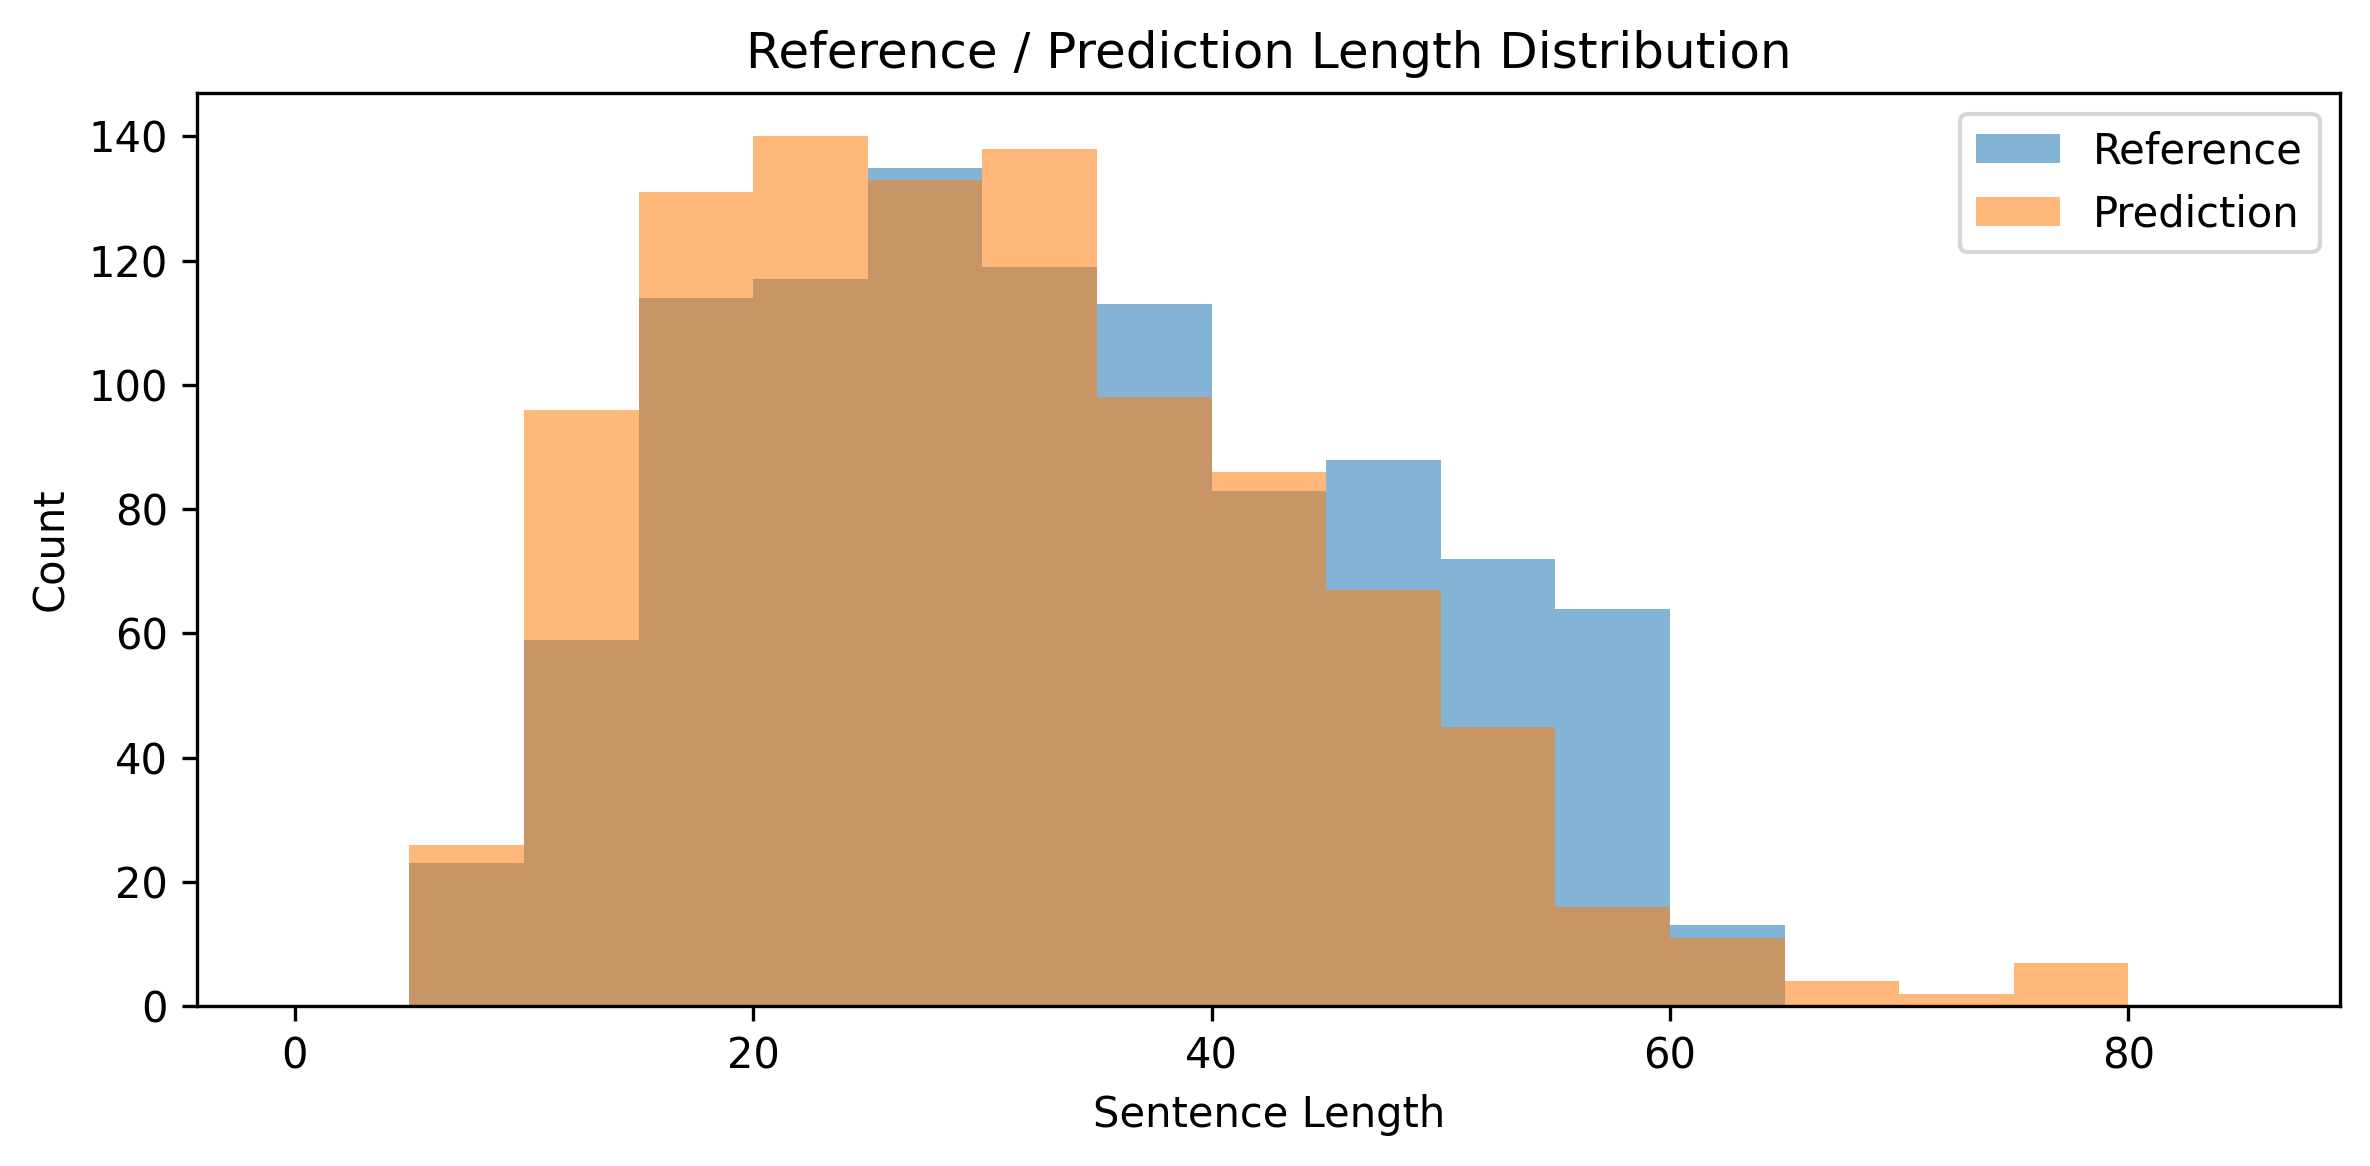
\includegraphics[width=0.76\linewidth]{../Figure/length_distribution.png}
		\caption{参考译文与模型译文长度分布}
	\end{figure}

	测试集源句平均长度为24.77，参考译文平均长度为32.88，模型译文平均长度为29.93。图3显示模型译文长度整体接近参考译文，但略短一些。这会通过BLEU中的brevity penalty产生一定惩罚，也说明模型有时会省略源句中的部分修饰信息或从句信息。

	\section{翻译样例与单句BLEU}
	整体BLEU-4为14.99，但一个总分不太容易看出模型到底翻译成了什么样子。这里选取4个测试句子，分别计算单句BLEU-4。单句BLEU比语料级BLEU更不稳定，尤其是短句中高阶$n$-gram本来就少，所以这些样例主要用来辅助观察模型输出。

	\begin{figure}[H]
		\centering
		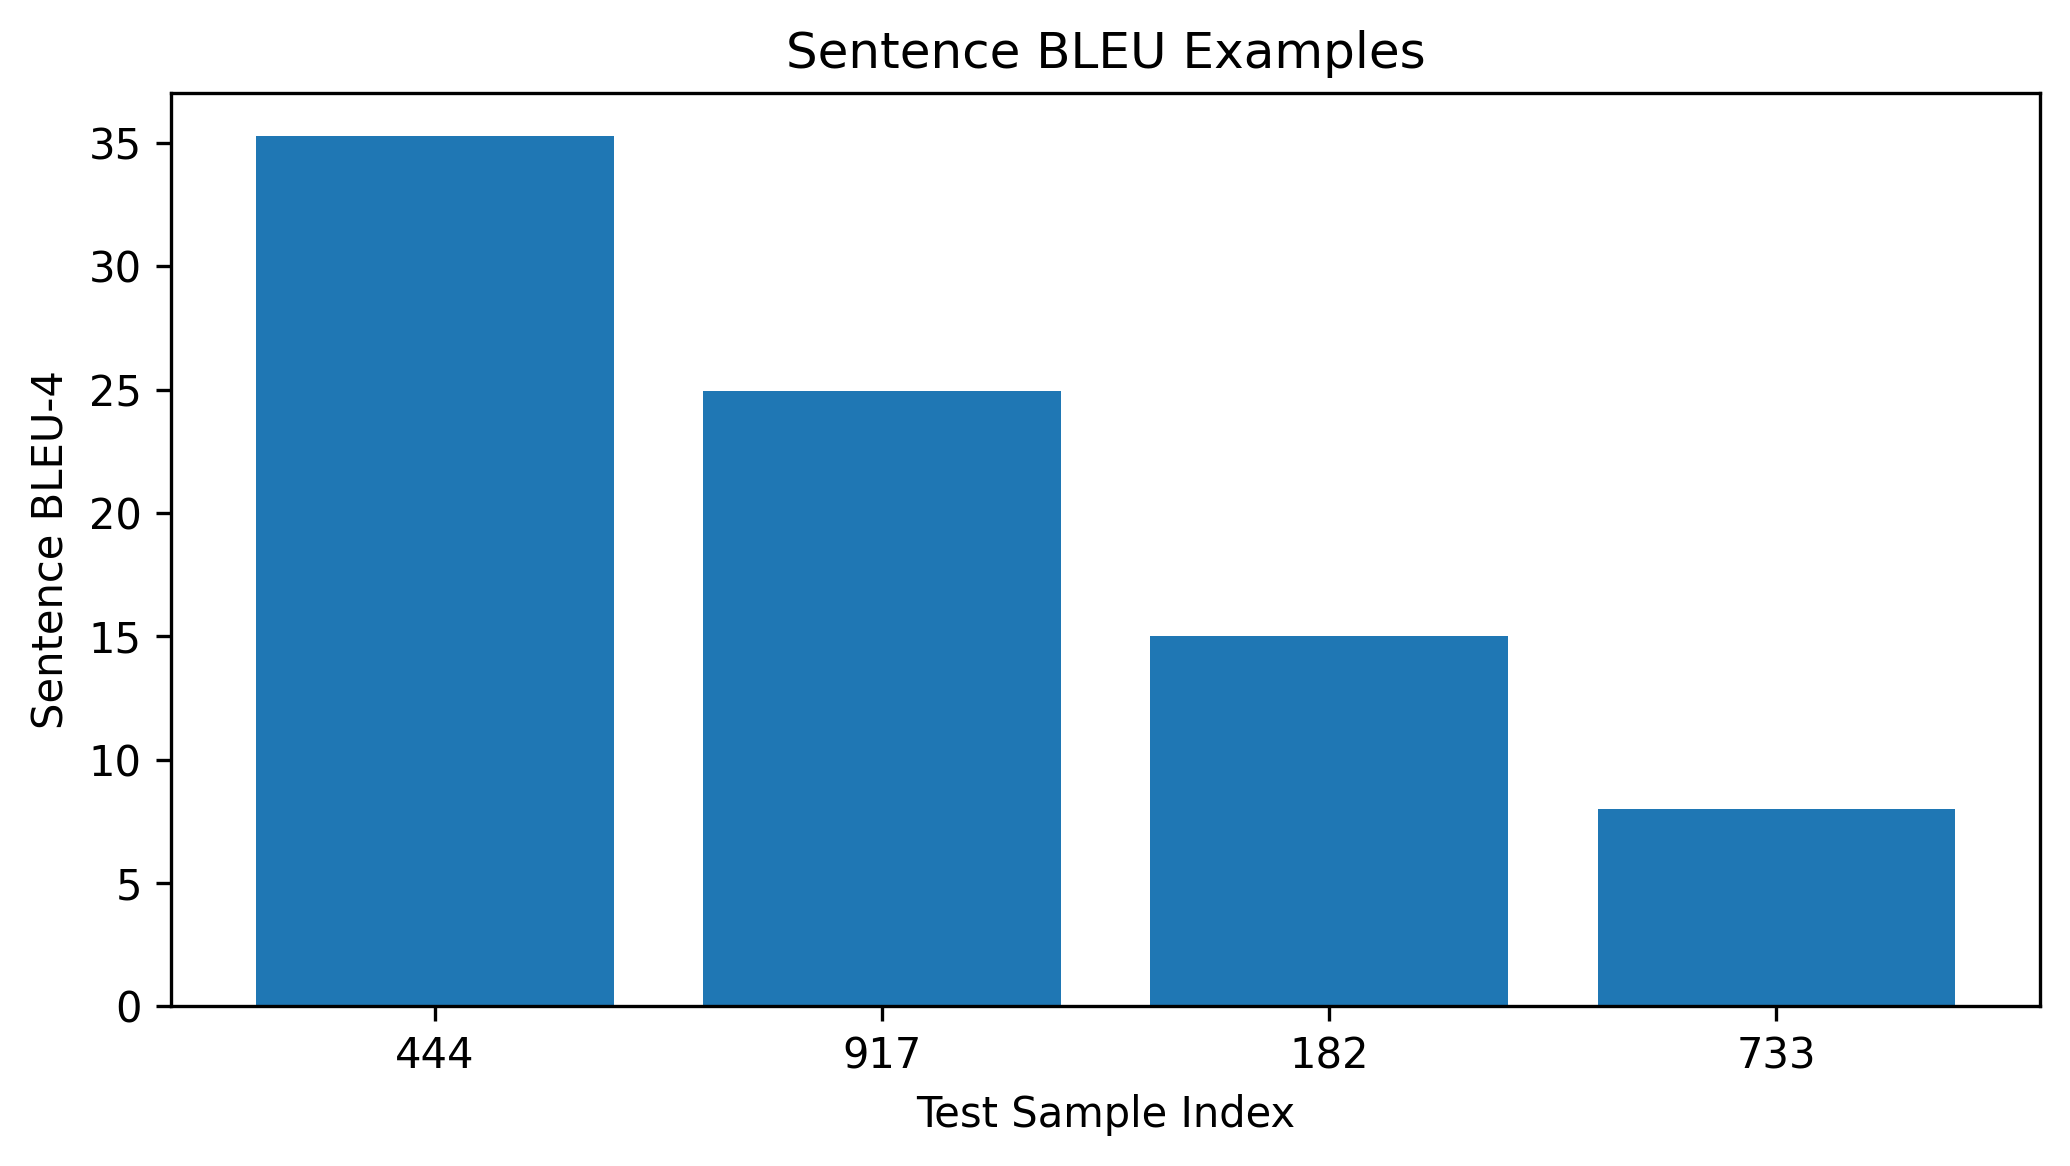
\includegraphics[width=0.68\linewidth]{../Figure/sentence_bleu_examples.png}
		\caption{样例句子的单句BLEU-4}
	\end{figure}

	\transbox{样例444，BLEU-4=35.27}
	{迟浩田 首先 转达 了 李鹏 委员长 对 布马扎 的 诚挚 问候 和 良好 祝愿 , 并 请 布马扎 转达 江泽民 主席 对 阿尔及利亚 总统 布特弗利卡 的 亲切 问候 和 良好 祝愿 .}
	{chi haotian first conveyed president jiang zemin 's cordial regards and best wishes to president bouteflika . he also asked chi haotian to convey his cordial regards and good wishes to president bouteflika .}
	{chi haotian first conveyed chairman li peng 's sincere regards and good wishes to boumaza and asked boumaza to convey president jiang zemin 's cordial and good wishes to algerian president abdelaziz bouteflika .}

	这个例子分数较高，主要是因为模型翻出了``迟浩田''、``江泽民''、``总统''和``良好祝愿''等关键词，很多外交文本中的高频表达也和参考译文接近。从模型角度看，这类句子在训练语料中应该比较常见，模型已经学到了一些固定模板，比如``conveyed ... regards and best wishes''。不过这个句子里人名较多，且有两层``转达''关系，模型把其中一部分人物关系混在了一起，后半句也重复生成了相似短语。这说明模型对常见表达掌握得较好，但遇到多个实体和多重指代时，Encoder表示和贪心解码仍然不够稳定。

	\transbox{样例917，BLEU-4=24.96}
	{近年来 , 该 研究所 取得 了 一大批 科技 创新 成果 , 为 我军 新型 导弹 武器 的 战斗力 建设 提供 了 强有力 的 技术 支持 .}
	{in recent years , the research institute of science and technology has provided a powerful support for our military 's technological achievements in the building of a large number of new type of weaponry .}
	{in recent years , the research institute attained a host of achievements in scientific and technological innovation , providing powerful technical support for the development of the combat effectiveness of new - type missiles and weapons .}

	这个例子保留了``近年来''、``研究所''、``科技''、``强有力支持''和``新型武器''等主要信息，所以BLEU不低。模型输出看起来像是抓住了句子的主题词，然后生成了一句比较顺的英文，但没有完整展开``取得科技创新成果''和``提供技术支持''这两个部分之间的关系。这里的问题更像是模型倾向于生成训练中常见的泛化表达，而不是逐项覆盖源句信息。由于当前使用的是贪心解码，一旦前面选中了比较宽泛的表达，后面就容易沿着这个方向继续生成，导致译文比参考答案更压缩。

	\transbox{样例182，BLEU-4=15.01}
	{结果 显示 , 董建华 的 民望 由 三月 的 五十九点一 , 急 跌至 五十二点九 , 跌幅 高达 前所未有 的 六点二 , 为 他 在 上任 以来 的 最低 位 .}
	{the results of his administration show that since the beginning of march , tung chee - hwa 's \texttt{<unk>} has been greatly \texttt{<unk>} .}
	{the results show that tung chee - hwa 's popularity plunged sharply from 59.1 points in march to 52.9 points , a drop of 6.2 points , falling to the lowest point since he took office .}

	这个句子里模型只抓住了``结果显示''、``董建华''和``三月''等片段，后面的数字变化和``最低位''没有翻出来，还出现了\texttt{<unk>}。这和词表构造方式有关：当前使用词级词表，低频词会被映射成\texttt{<unk>}，数字和政治新闻中的专有表达也比较容易被截断。模型一旦在关键位置生成\texttt{<unk>}，后续解码就会缺少明确语义线索，因此后半句变得很短。这个例子反映出词级NMT在低频词、数字和专名上不如子词模型稳。

	\transbox{样例733，BLEU-4=7.99}
	{若 如此 , 还需要 什 麽 神 盾 舰 ?}
	{if the aegis combat system is so advanced , what kind of aegis combat will be ?}
	{then why do we need aegis ships ?}

	这个短句的参考译文很简洁。模型识别出了``aegis''，但把``神盾舰''扩展成了``aegis combat system''一类表达，译文变长后意思也偏了一些。从模型角度看，短句给Encoder提供的上下文较少，模型更依赖训练集中和``aegis''一起出现的常见搭配；贪心解码又会每一步选择当前概率最大的词，所以容易生成局部常见但整体不贴合源句的短语。短句本来可匹配的4-gram就很少，这种偏差会让单句BLEU降得很明显。

	\section{总结}
	本次实验实现了一个基于Transformer的中英神经机器翻译系统，完成了数据读取、词表构造、数值化缓存、Encoder-Decoder模型、teacher forcing训练、贪心解码和BLEU-4评估。最终模型在测试集上得到BLEU-4为14.99，达到实验指导书中BLEU-4大于14的要求。

	从实验过程看，模型已经学到了一些新闻和外交文本里的常见表达，对高频词、固定短语和简单句式翻译得还可以。但复杂长句、低频词、数字和专有名词仍然会带来问题，\texttt{<unk>}和信息遗漏也还存在。译文平均长度略短于参考译文，说明模型有时会生成偏保守的句子。后续如果继续优化，可以考虑使用子词级分词减少\texttt{<unk>}，或者引入beam search和长度惩罚来改善解码。

	\begin{thebibliography}{9}
		\bibitem{papineni2002bleu}
		Kishore Papineni, Salim Roukos, Todd Ward, and Wei-Jing Zhu.
		\newblock BLEU: a Method for Automatic Evaluation of Machine Translation.
		\newblock In \emph{Proceedings of the 40th Annual Meeting of the Association for Computational Linguistics}, 2002.
		\newblock \url{https://dl.acm.org/doi/10.3115/1073083.1073135}
	\end{thebibliography}

\end{document}
